\documentclass{beamer}

\usepackage{beamerthemesplit}

\title{CA in graphics}
\author{Walter Schulze}
\date{\today}

\begin{document}

\frame{\titlepage}

\section[Outline]{}
\frame{\tableofcontents}

\section{Introduction}
\frame
{
  \frametitle{Introduction}
  \begin{itemize}
  \item<1-> Simulation of Clay
  \item<2-> Plate pushing down
  \item<3-> Distribution of Clay
  \end{itemize}
}
\frame
{
	\frametitle{2D Margolus Area}
	\begin{figure}[htbp]
   \centering
   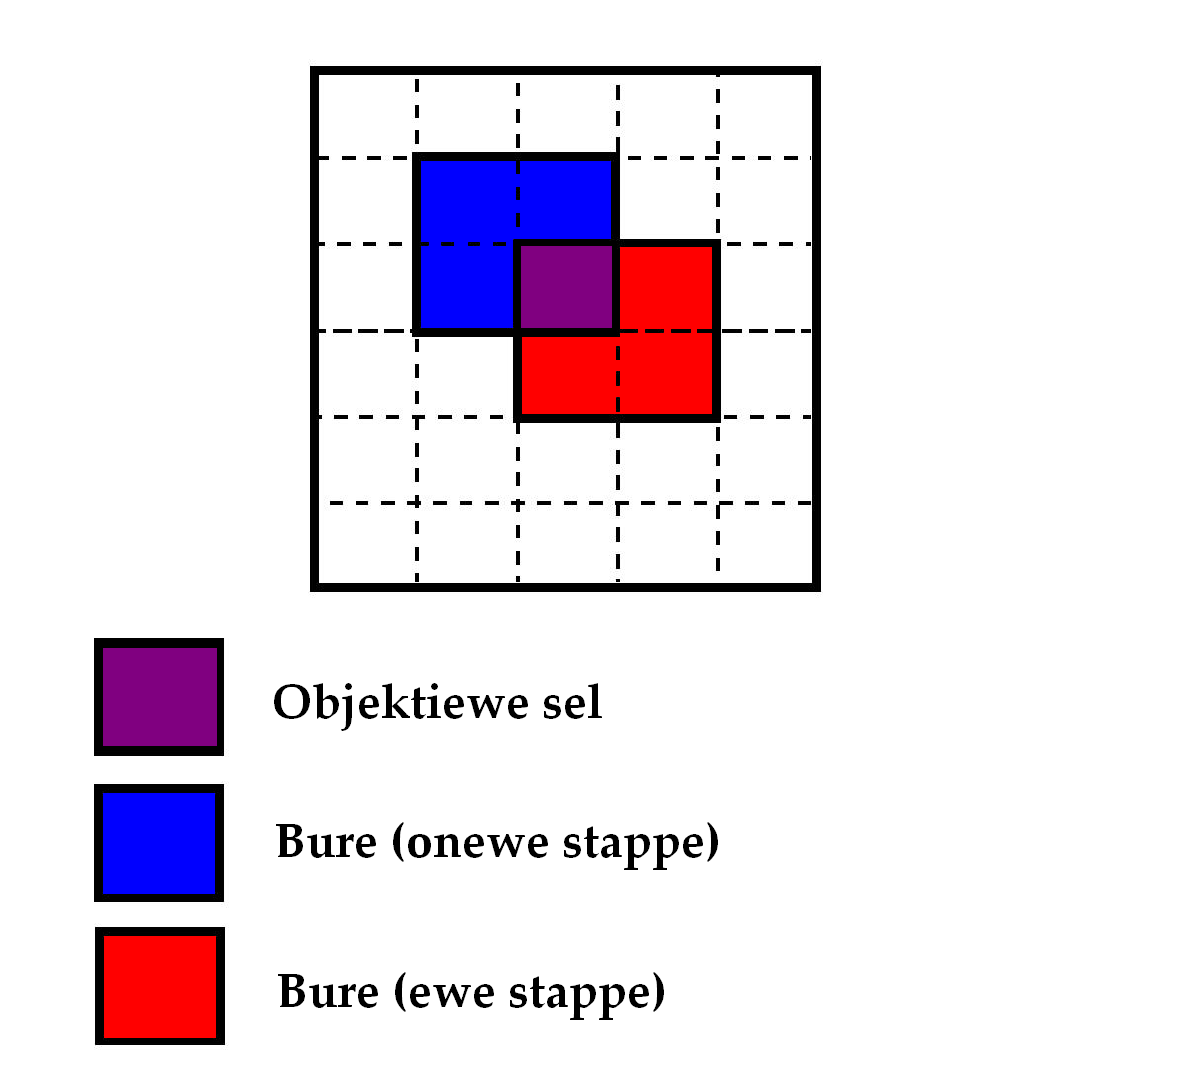
\includegraphics[width=5cm]{bure4.png}
   \caption{2D Margolus Area}
   \label{Figure:figex}
	\end{figure}
}
\frame
{
	\frametitle{Active Areas}
	\begin{figure}[htbp]
	   \centering
	   \includegraphics[width=3cm]{omgewing2.png}
	   \caption{Even and Uneven sized matrixes}
	   \label{Figure:figex}
	\end{figure}
}
\frame
{
	\frametitle{Plate pushing down}
	\begin{figure}[htbp]
   \centering
   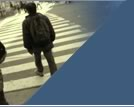
\includegraphics[width=9cm]{pic3.png}
   \caption{Clay pillar begin pushed on by plate}
   \label{Figure:figex}
	\end{figure}
}
\section{Implimentation}
\frame
{
	\frametitle{Input format}
	size=100=100 \\
	threshold=10 \\
	start=5 \\
	random=5 \\
	pillar=25=75=50=100 \\
	press=15=70=40 \\
	pause=0 \\
	alfa=0=0.3 \\
}
\frame
{
	\frametitle{Time Complexity}
	\begin{itemize}
	\item<1-> moving clay = O(2(x-1)(y-1)) not O(2xy) and not O((x-1)(y-1))
	\item<2-> moving plate = O((x(y-1)+3L) 
	\item<3-> graphics = O(xy) 
	\item<4-> total = O(2(x-1)(y-1) + x(y-1)+3L + xy)
	\item<5-> approximately = O(4xy) 
	\end{itemize}
}
\frame
{
	\frametitle{Factor of threshold and alpha}
	\begin{figure}[htbp]
   \centering
   \includegraphics[width=8cm]{graph2.png}
   \caption{threshold and alpha against tyd}
   \label{Figure:figex}
	\end{figure}
}
\section{Testing}
\frame
{
	\frametitle{Testing example}
	\begin{figure}[htbp]
   \centering
   \includegraphics[width=8cm]{pic5.png}
   \caption{3 plates without random clay}
   \label{Figure:figex}
	\end{figure}
}
\section{Summary}
\frame
{
	\frametitle{Summary}
	Fun and easy use of Cellular Automata 
	
	Computation time for each cycle is approximately O(4xy) 
	
	Alpha and Threshold the bigger the more fluid like the clay is 
}
\section{Bibliography}
\frame
{
	\frametitle{Bibliography}
	Efficient Cellular Automata for 2D / 3D Free-Form Modeling 
	authors: S. Druon, A. Crosnier en L. Brigandat 
	webiste: http://wscg.zcu.cz/wscg2003/Papers 2003/I17.pdf 
	
}
\end{document}
